\chapter{相关技术与理论基础}

\section{词向量表示}

词嵌入(Word embedding)是文档词汇最流行的表示形式之一,它是特定单词的向量表示,它能够捕获文档中单词的上下文,语义和句法相似性,与其他单词的关系等。
Word2Vec是使用浅层神经网络学习单词嵌入的最流行技术之一,它是由Tomas Mikolov于2013年在Google上提出的。
Word2Vec是一个浅层的两层神经网络,经过训练可以重建单词的上下文语义。 它的输入来源是一个大的单词语料库,通常产生一个具有几百个维度的向量空间,
该语料库中的每个唯一单词都在该空间中分配了一个相应的向量。 词向量位于向量空间中,以便在语料库中共享公共上下文的词在空间中彼此紧邻。 

  Word2Vec是具有单个隐藏层的简单神经网络,并且像所有神经网络一样,它具有权重,并且在训练过程中,其目标是调整这些权重以减少损失函数。 
  但是,Word2Vec不是用于他训练时处理的任务,相反,我们将仅使用其隐藏的权重,将其用作词嵌入,然后将模型的其余部分扔掉。
  这个trick在无监督的特征学习中也有用到,其中训练了自编码器以在隐藏层中压缩输入向量,然后将其解压缩回输出层中的原始向量,
  训练完成后,剥离输出层,仅使用隐藏层,因为它学习了良好的编码功能。
  如果不同的单词在上下文中相似,那么当这些单词作为输入传递时,Word2Vec应该具有相似的输出,
  并且为了具有相似的输出,这些单词在隐藏层中计算出的单词矢量必须相似,因此Word2Vec的动机是为相似上下文中的单词学习相似的单词向量。
Word2Vec能够捕获单词之间的多个不同程度的相似度,从而可以使用词向量来表示语义和句法模式。
可以通过对这些单词的词向量进行代数运算来生成诸如“男人之于女人等于兄弟之于姐妹”的模式,
从而使“兄弟”-“男人” +“女人”的词向量与“姐妹”的词向量表示十分接近,如图\ref{fig:linear-relationships}所示。


\begin{figure}[htbp]
  \centering
  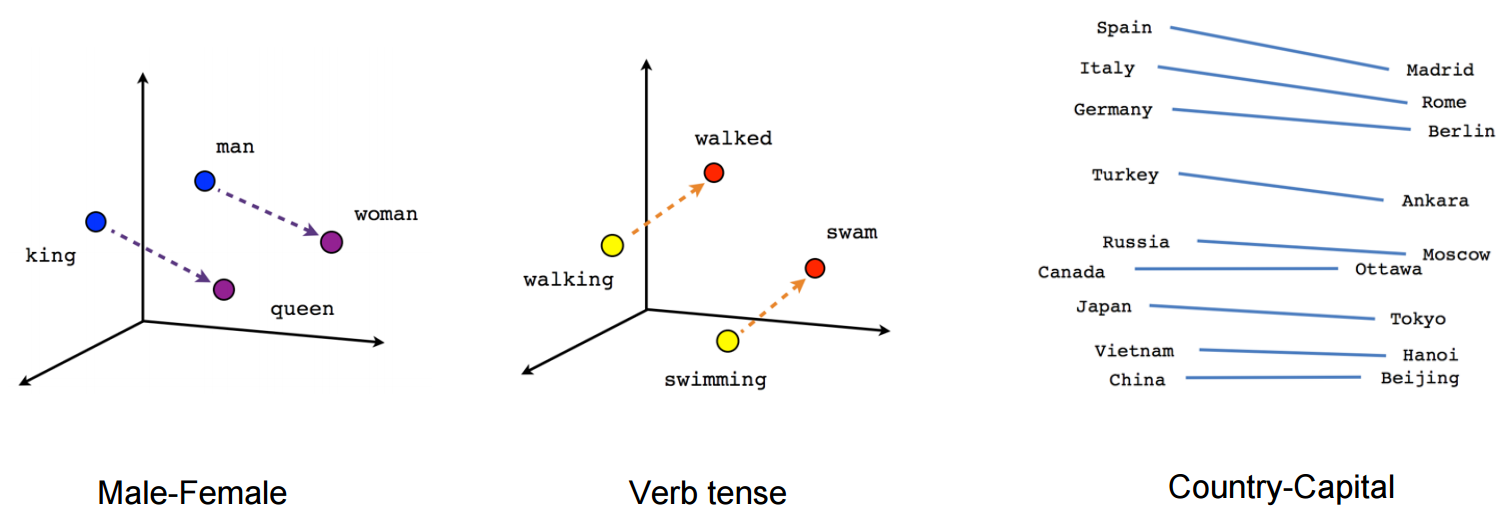
\includegraphics[scale=0.5]{./images/linear-relationships.jpg}
  \caption{词向量之间关系}
  \label{fig:linear-relationships}
\end{figure}


  Word2Vec是一种从原始文本中学习单词嵌入的计算效率特别高的预测模型,
它主要有两种方式,连续词袋(CBOW)模型和Skip-Gram模型,如图\ref{fig:word2vec_diagrams}。
\begin{figure}[htbp]
  \centering
  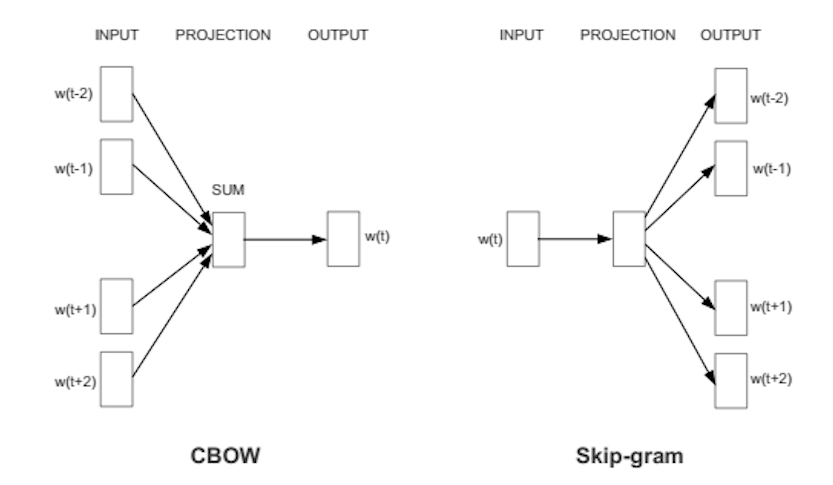
\includegraphics[scale=0.5]{./images/word2vec_diagrams.png}
  \caption{word2vec两种训练方式}
  \label{fig:word2vec_diagrams}
\end{figure}
CBOW模型:此方法将每个单词的上下文作为输入,并尝试预测与上下文相对应的单词。
如图\ref{fig:CBOW}的模型采用C个上下文词,输入是他们的onehot表示,乘以共享矩阵W(维度是V*N)求均值
得到的结果作为隐藏层,是一个N维的矩阵,隐藏层向量乘以输出权重矩阵W'得到输出向量,即为从上下文
中扣出的单词。


\begin{figure}[htbp]
  \centering
  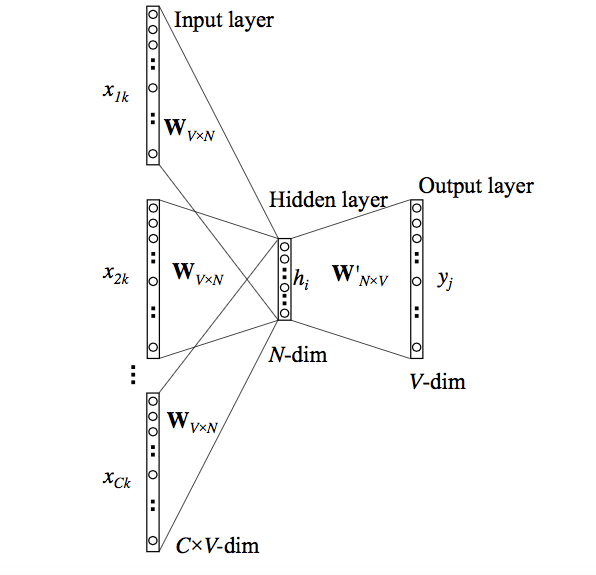
\includegraphics[scale=0.4]{./images/CBOW.jpg}
  \caption{CBOW}
  \label{fig:CBOW}
\end{figure}


给定一个单词,Skip-gram模型的伪造任务是尝试预测其相邻单词,可以简单的看作将cbow模型反过来。

\begin{figure}[htbp]
  \centering
  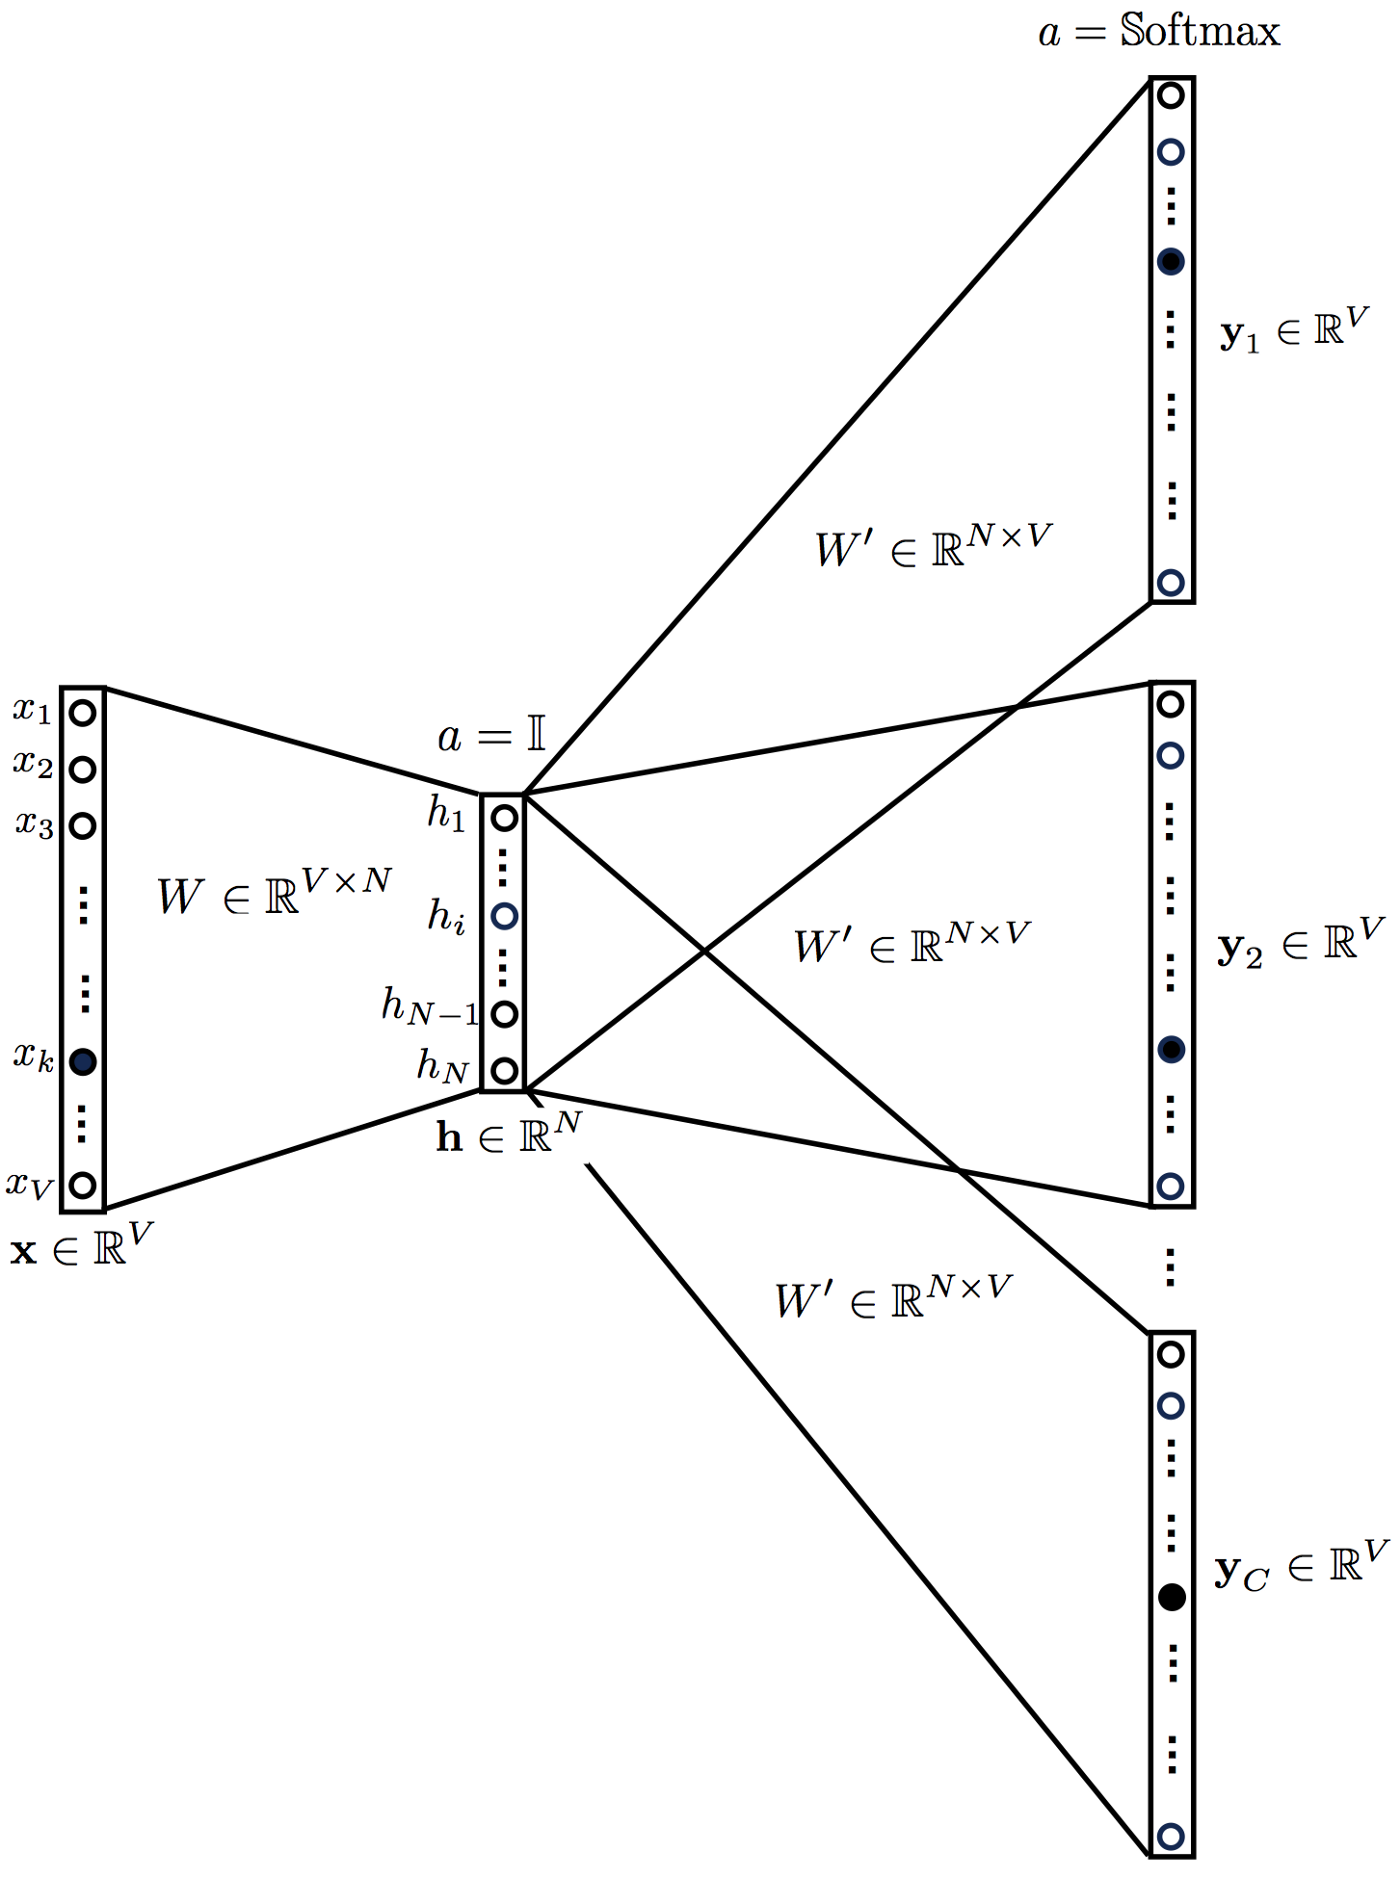
\includegraphics[scale=0.15]{./images/skip.jpg}
  \caption{skip-gram}
  \label{fig:skip}
\end{figure}

\section{循环神经网络}

\subsection{RNN}

循环神经网络(RNN)是一种神经网络,其中前一步的输出将作为输入输入到当前步骤。在传统的神经网络中,
所有输入和输出都是彼此独立的,但是在例如需要预测句子的下一个单词的情况下,需要前一个单词,
因此需要记住前一个单词。因此,RNN诞生了,它借助“隐藏层”解决了这个问题。
RNN的主要和最重要的功能是“隐藏状态”,它可以记住一些有关序列的信息。

RNN有一个“内存”,可以记住有关已计算内容的所有信息。它对每个输入使用相同的参数,
因为它在所有输入或隐藏层上执行相同的任务以产生输出,与其他神经网络不同,这降低了参数的复杂性。
RNN通过为所有层提供相同的权重和偏差将独立激活转换为相关激活,
从而通过将每个输出作为下一个隐藏层的输入来降低增加参数的复杂性并存储每个先前的输出。

\begin{figure}[htbp]
  \centering
  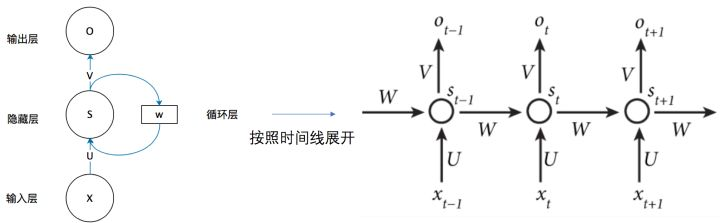
\includegraphics[scale=0.5]{./images/rnn.jpg}
  \caption{RNN}
  \label{fig:rnn}
\end{figure}

上图\ref{fig:rnn}显示了将RNN 展开为完整的网络,rnn可以被我们展开为我们想要的任意层数。例如,
如果我们关心的序列是5个单词的句子,则该网络将展开为5层神经网络,每个单词一层。对于上图具体来说,
$x_{t}$是时刻t的输入,例如,$x_{1}$ 可以是与句子的第二个单词相对应的one-hot向量。
$s_{t}$是时刻t的隐藏状态,这是网络的“记忆”,$s_{t}$根据先前的隐藏状态和当前步骤的输入来计算

\begin{equation}
  s_{t}=f(U x_{t}+W s_{t-1})
  \end{equation}

该函数f通常是诸如tanh或ReLU之类的非线性函数,$s_{-1}$计算第一个隐藏状态所需的,通常初始化为全零。
$o_{t}$是时刻t的输出,例如,如果我们想预测句子中的下一个单词,那么它将是整个词汇表中单词的概率分布
\begin{equation}
  o_t = \mathrm softmax (V s_t)
  \end{equation}

  你可以将隐藏状态$s_{t}$视为网络的记忆,$s_{t}$捕获有关先前时间步中发生的所有情况的信息。步骤t的输出$o_{t}$仅基于时间t的记忆进行计算,
  但是在实际情况中会有点问题,因为$s_{t}$通常无法从太早时间之前捕获信息。与传统的深度神经网络在每一层使用不同的参数不同,
  RNN图中U,V,W在所有步骤中共享相同的参数。这是因为我们在每个步骤都执行相同的任务,只是输入的内容不同,这大大减少了我们需要学习的参数总数。
  上图在每个时间步都有输出,但是根据任务的不同,可能有些是没有必要的。例如,在预测句子的情感时,我们可能只关心最终的输出,而不关心每个单词的情感。
  同样,我们可能不需要每个时间步都输入。RNN的主要特征是其隐藏状态,该状态能够捕获有关序列的一些信息。


  
  \subsection{LSTM}
  RNN的优势在于它可以将先前的信息连接到当前任务,例如使用先前的视频帧可能会有助于对当前帧的理解。考虑一种语言模型,该模型试图根据前一个单词预测下一个单词。
  如果我们试图预测“the clouds are in the sky”的最后一个词,则不需要任何进一步的上下文,很明显,下一个词将是“sky”,
  在这种情况下,如果相关信息与所需信息之间的差距很小,则RNN可以很好的学习使用过去的信息。
  但是在某些情况下,我们需要更多的上下文。考虑尝试预测文本“I grew up in France… I speak fluent French.”中的最后一个词。
  最近的信息表明,下一个词可能是一种语言的名称,但是如果我们想缩小哪种语言的范围,我们需要从更远的地方来追溯法国的情况。相关信息与这些相关信息被需要的地方之间的差距很大是完全可能的,
不幸的是,随着差距的扩大,RNN变得无法学习连接信息。

长短期记忆网络(通常称为“ LSTM”)是一种特殊的RNN,能够学习长期依赖关系,它是由Hochreiter&Schmidhuber(1997)提出的,
并在随后的工作中被许多人改进和推广,它在各种问题上都表现出色,现已被广泛使用。
LSTM被明确设计为避免长期依赖问题,长时间记住信息实际上是他的默认行为,而不是他努力学习的东西。
所有的递归神经网络都具有神经网络的重复模块链的形式,在标准RNN中,此重复模块将具有非常简单的结构,例如单个tanh层。
LSTM也具有这种链状结构,但是重复模块具有与传统rnn不同的结构,它不是只有一个神经网络层,而是有四个,以非常特殊的方式进行交互。

\begin{figure}[htbp]
  \centering
  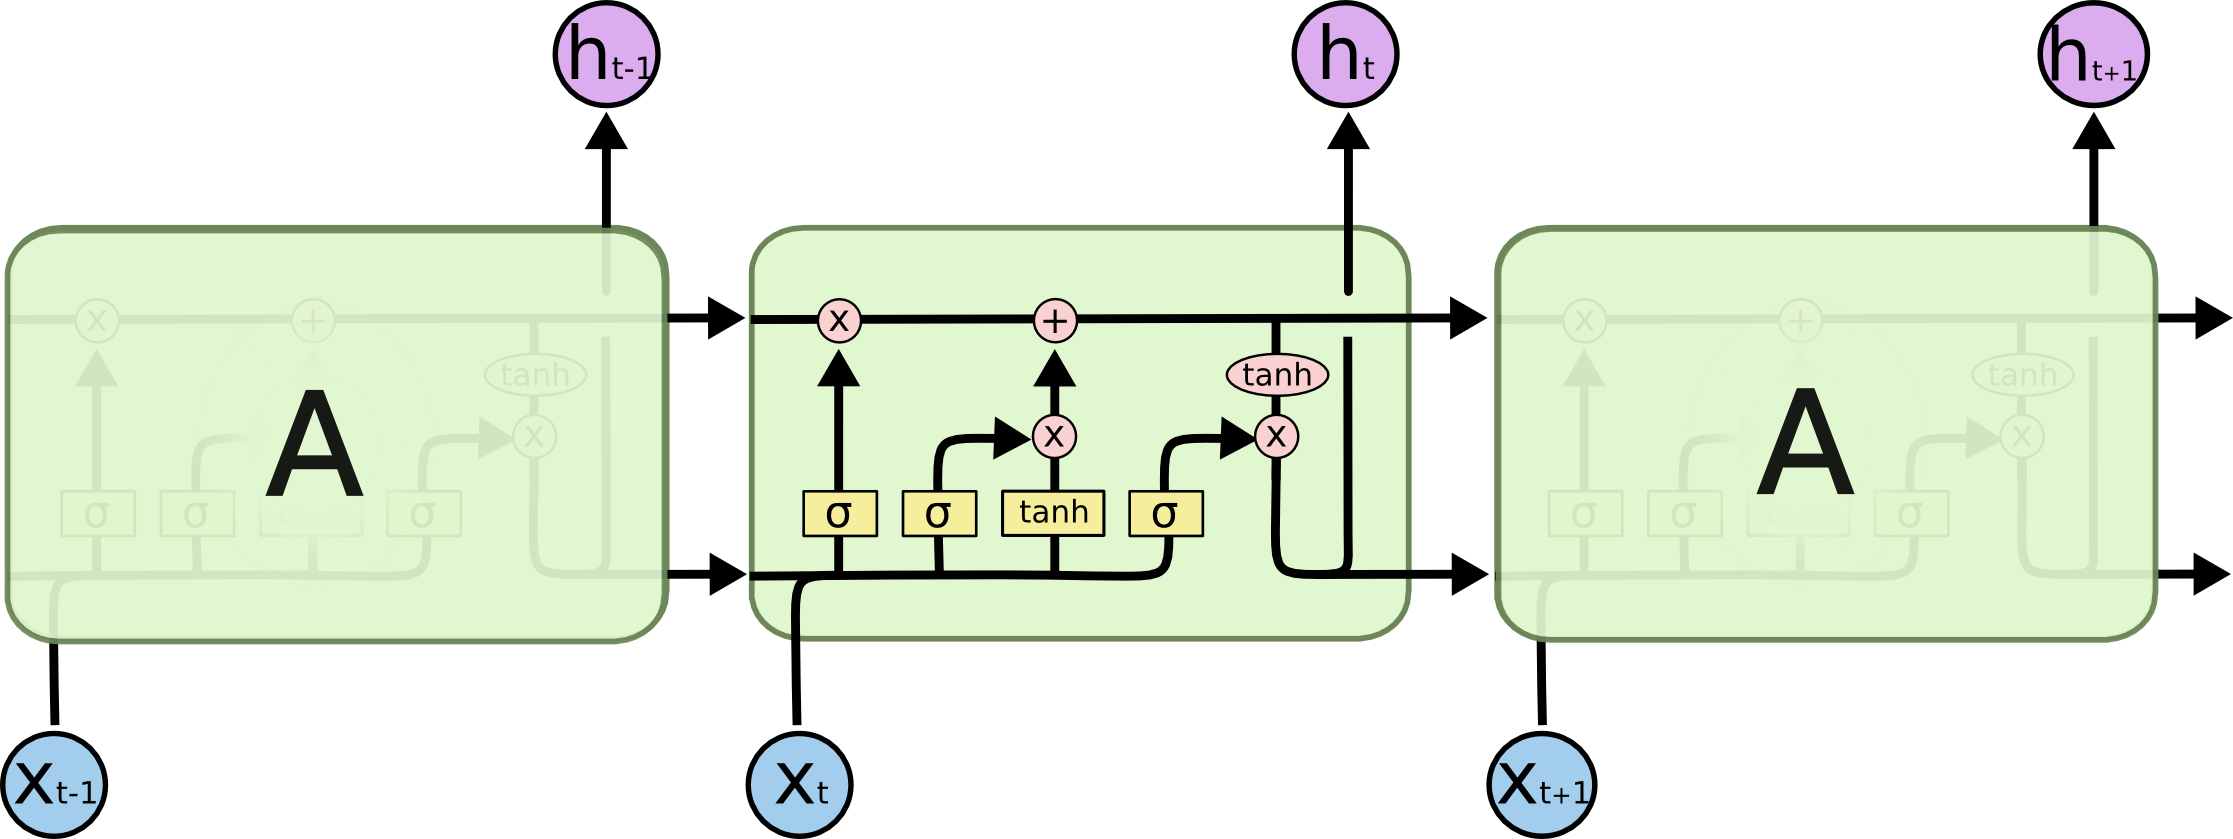
\includegraphics[scale=0.5]{./images/LSTM.jpg}
  \caption{LSTM中的重复模块包含四个交互层}
  \label{fig:LSTM}
\end{figure}

LSTM的关键是cell状态,水平线贯穿图的顶部。单元状态有点像传送带。它沿整个链条一直沿直线延伸,只有一些较小的线性相互作用,信息能够非常容易地不加改变地流动。
LSTM具有删除或向单元状态添加信息的能力,这些功能由称为门的结构精心调节,Gates是一种选择性地让信息通过的方式,它由sigmoid神经网络层和点乘运算组成。
sigmoid输出介于零和一之间的数字,描述应允许每个组件中的多少通过。值为零表示“不让任何内容通过”,而值为1表示“让所有内容通过”。
LSTM的第一步是确定要从单元状态中丢弃的信息。该决定由称为“忘记门层”的sigmoid层决定。它输入$h_{t-1}$和$x_{t}$,并对于单元格$c_{t-1}$状态中的每个数字输出一个介于 0 和 1的值,
1表示“完全保留此”,而 0 表示“完全摆脱这一点”。
\begin{equation}
  f_{t}=σ(W_{f}\cdot[h_{t-1},x_t]+b_{f})
  \end{equation}

  下一步是确定要在cell状态下存储哪些新信息,这包括两个部分。首先,一个称为“输入门层”的sigmoid层决定了我们将更新哪些值。
  接下来,tanh层创建一个新候选值的向量$\tilde{C}_{t}$,可以将其添加到状态中。在下一步中,我们将两者结合起来以创建状态更新。
  \begin{equation}
    i_{t} =\sigma\left(W_{i} \cdot\left[h_{t-1}, x_{t}\right]+b_{i}\right) 
  \end{equation}  
    \begin{equation}
      \tilde{C}_{t} =\tanh \left(W_{C} \cdot\left[h_{t-1}, x_{t}\right]+b_{C}\right)
      \end{equation}   

现在该更新旧单元格状态$C_{t-1}$,进入新的单元状态$C_{t}$。前面的步骤已经确定了要做什么,我们只需要执行即可。
我们将旧状态乘以 $f_{t}$,忘记我们决定早点忘记的事情,然后我们添加$i_{t} * \tilde{C}_{t}$,这是新的候选值,
根据此决定我们更新每个状态值的大小。
\begin{equation}
C_{t}=f_{t} * C_{t-1}+i_{t} * \tilde{C}_{t}
\end{equation} 

最后,我们需要决定要输出的内容。此输出将基于我们的cell状态,但将是过滤后的版本。
首先,我们运行一个sigmoid层,该层决定要输出的单元状态的哪些部分。
然后,我们通过tanh(将值推到介于 − 1 和 1),然后将其乘以sigmoid层的输出,这样我们就只输出我们决定的部分。
\begin{equation}
  o_{t}=\sigma\left(W_{o}\left[h_{t-1}, x_{t}\right]+b_{o}\right)
\end{equation} 
\begin{equation}
  h_{t}=o_{t} * \tanh \left(C_{t}\right)
\end{equation}



\section{预训练模型}
\subsection{seq2seq}
\subsection{attention}
\subsection{transformer}
\subsection{bert}
NLP的最大挑战之一是缺乏足够的训练数据,从全局视角来看有大量的文本数据可用,但是如果我们要创建特定任务的数据集,则需要将总的数据堆划分为很多不同的小块。
而当我们这样做时,我们最终仅得到数千或数万个人为标记的培训示例。不幸的是,为了表现良好,基于深度学习的NLP模型需要大量的数据,在数百万或数亿的带注释的训练样本上进行训练时,
模型效果相比少数据量会有质的提升。为了帮助弥合数据鸿沟,研究人员开发了多种技术,可在网络上使用大量无注释的文本来训练通用语言表示模型(这称为预训练),
然后,可以在较小的特定任务的数据集上微调这些通用的预训练模型,例如,在处理诸如问答系统和情感分析之类的问题时。与从头开始对较小的特定于任务的数据集进行训练相比,
此方法可显着提高准确性。BERT是这些技术中用于NLP预训练的最新功能,它在深度学习社区引起了轰动,因为它在各种NLP任务中都提供了最优异的成果。

语言建模的真正意义是什么?语言模型试图解决哪些问题?基本上,他们的任务是根据上下文“填补空白”。例如,给定
“The woman went to the store and bought a( )of shoes”,语言模型可能会说“cart”一词将在20%的情况合适,而“pair”一词将在80%的情况合适。
在BERT之前的世界中,语言模型会在训练期间从左到右或从左到右和从右到左的组合查看此文本序列。这种单向方法很适合生成句子,我们可以预测下一个单词,
将其附加到序列中,然后预测下一个单词的下一个单词,直到获得完整的句子。
现在进入BERT时期,这是一种经过双向训练的语言模型(这也是其关键的技术创新),这意味着与单向语言模型相比,我们现在可以对语言上下文和流程有更深刻的了解。
BERT并没有预测序列中的下一个单词,而是使用了一种称为Masked LM(MLM)的新颖技术:它随机屏蔽句子中的单词,然后尝试预测它们。
掩蔽意味着该模型从两个方向看,并且它使用句子的整个上下文(左右环境)来预测被掩盖的单词。与以前的语言模型不同,它同时考虑了上一个和下一个词 。
基于LSTM的从左到右和从右到左组合的现有模型缺少此能力。(不过,说BERT是无方向性的可能更准确。)

但是,为什么这种非定向方法如此强大?预训练的语言表示可以是上下文无光或基于上下文的。上下文相关的模型又可以分为单向和双向的。
word2vec之类的上下文无关模型会为词汇表中的每个单词生成单个单词嵌入表示(数字矢量)。
例如,单词“bank”在“bank account”和“bank of the river”中将具有相同的上下文无关表示。
另一方面,基于上下文的模型会基于句子中的其他单词生成每个单词的表示形式。例如,在句子““I accessed the bank account”,
单向上下文模型将基于“I accessed the”而不是“account”来表示“bank” 。但是,BERT从前部和后部上下文信息(“I accessed the … account”)表示“bank”,
它从深度神经网络的最底层开始,使其深度双向化。

BERT依赖于Transformer(一种学习文本中单词之间的上下文关系的注意力机制),一个基本的Transformer由一个读取文本输入的编码器和一个对任务进行预测的解码器组成。
由于BERT的目标是生成语言表示模型,因此只需要编码器部分即可。BERT编码器的输入是一系列token,这些token首先被转换为矢量,然后在神经网络中进行处理。
但是在开始处理之前,BERT需要对输入进行处理并用一些额外的元数据修饰:

1.令牌嵌入:在第一个句子的开头将[CLS]令牌添加到输入的单词令牌中,并在每个句子的末尾插入[SEP]令牌。

2.段嵌入:将指示句子A或句子B的标记添加到每个标记,这使编码器能够区分句子。

3.位置嵌入:将位置嵌入添加到每个标记,以指示其在句子中的位置。
\begin{figure}[htbp]
  \centering
  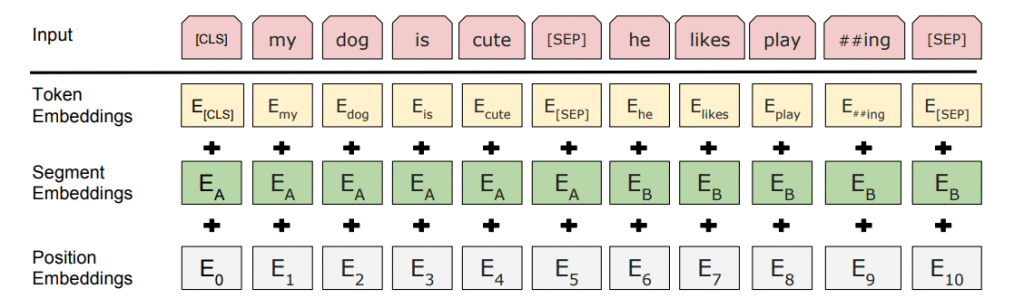
\includegraphics[scale=0.5]{./images/inputBert.jpg}
  \caption{bert的输入处理}
  \label{fig:inputBert}
\end{figure}

本质上,Transformer会堆叠一个将序列映射到序列的层,因此输出也是在相同索引处的输入和输出令牌之间具有一一对应关系的向量序列。
而且正如我们之前所了解的,BERT不会尝试预测句子中的下一个单词。培训使用以下两种策略:Masked LM (MLM),这里的想法是简单的,
随机掩盖输入中15%的单词(用[MASK]令牌代替),通过基于BERT注意的编码器运行整个序列,然后根据序列中其他未屏蔽单词提供的上下文预测被屏蔽的词,
但是,这种掩盖方法存在一个问题,模型仅尝试预测输入中存在的词,而我们希望模型尝试预测正确的token,而不管该token是否存在输入中。
要解决此问题,bert在训练时,实际上有80%的tokenb被替换为令牌[MASK],10%的令牌被替换为随机令牌,10%的令牌保持不变。Next Sentence Prediction,
为了理解两个句子之间的关系,BERT训练过程还使用下一个句子预测,具有这种理解的预训练模型与诸如回答问题之类的任务有关。
在训练过程中,该模型将句子对作为输入,并学习预测第二个句子是否是原始文本中的下一个句子。第二句出现在第一句之后的概率有50%,剩下50%出现的是语料库中随机的句子。
为了预测第二句话是否与第一句话相连,基本上整个输入序列都会经过基于Transformer的模型,使用简单的分类层将[CLS]令牌的输出转换为2×1形状的矢量,
并使用softmax分配IsNext-Label。